\documentclass[a4paper,12pt]{article}
\usepackage[indonesian]{babel}
\usepackage{graphicx}
\usepackage{multirow}
\usepackage{enumitem}
\usepackage{listings}
\usepackage{wrapfig}
\usepackage[T1]{fontenc}
\usepackage{inconsolata}
\usepackage{lipsum}
\usepackage{adjustbox}


\usepackage{color}
\usepackage[table]{xcolor}
\definecolor{mygreen}{rgb}{0,0.6,0}
\definecolor{mygray}{rgb}{0.5,0.5,0.5}
\definecolor{mymauve}{rgb}{0.58,0,0.82}
\lstset{%
    language=java,
    showstringspaces=false,          % Prevent tex replacing space to bracket in code
    frame=single,                    % Set frame around code
    backgroundcolor=\color{white},   % choose the background color
    basicstyle=\footnotesize,        % size of fonts used for the code
    breaklines=true,                 % automatic line breaking only at whitespace
    captionpos=b,                    % sets the caption-position to bottom
    commentstyle=\color{mygreen},    % comment style
    keywordstyle=\color{blue},       % keyword style
    stringstyle=\color{mymauve},     % string literal style
}

\graphicspath{ {./img/} }
\begin{document}
\title{ {\Large Laporan Praktikum}\\ Algoritma dan Pemrograman Lanjut\\{\Large Pertemuan 6}}

\author{Aldzikri Dwijayanto Prathama
    \\195410189
    \\Informatika}
\makeatletter
\begin{titlepage}
    \begin{center}
        {\huge \bfseries \@title}\\[14ex]
        
\includegraphics[scale=.8]{logo}\\[4ex]
        {\large \@author}\\[12ex]
        {\large \bfseries {SEKOLAH TINGGI MANAJEMEN INFORMATIKA DAN KOMPUTER
            AKAKOM YOGYAKARTA}}
    \end{center}


%{\large \@date}
\end{titlepage}
\makeatother
%\maketitle
\newpage
\tableofcontents
\newpage

\section{Tujuan}
\paragraph{}
Mahasiswa dapat:
\begin{enumerate}
Mahasiswa dapat menggabungkan konsep perulangan dalam seleksi bertingkat untuk menyelesaikan kasus
\end{enumerate}


\section{Teori}
\paragraph{}
Seleksi sudah dibahas pada Algoritma dan Pemrograman dengan seleksi tunggal dan ganda.
Seleksi digunakan untuk mengarahkan suatu proses itu berjalan. Seleksi adalah suatu program
untuk mengambil keputusan berdasarkan suatu kondisi. Seleksi ada dua macam bentuk
pernyataan. Seleksi dengan if \ldots else dan switch \ldots case.
Perulangan juga telah dibahas pada algoritma dan pemrograman serta untuk perulangan
bertingkat sudah dibahas pada pertemuan ke 2.: Perulangan (atau yang disebut Looping) adalah
suatu proses yang diklakukan secara berulang-ulang hingga mencapai kondisi tertentu.
Selanjutnya untuk permasalahan yang lebih komplek kita dapat menggabungkan konsep
seleksi dengan perulangan. Jika pada algoritma dibahas mengenai perulangan dalam seleksi
maka pada pada algoritmmma dan pemrograman lanjut ini dibahas mengenai perulangan dalam
seleksi bertingkat.
\newpage

\section{Pembahasan}
\subsection{Praktik}
\subsubsection{Praktik 1}
\begin{lstlisting}
import java.util.Scanner;

public class Praktik6_1 {
    public static void main(String args[]) {
        Scanner masuk = new Scanner(System.in);
        int nilai, i;
        System.out.println(" Masukan pilihan");
        System.out.println(" 1. bil ganjil");
        System.out.println(" 2. bil genap");
        System.out.print(" pilihan : ");
        nilai = masuk.nextInt();
        if (nilai == 1) {
            for (i = 1; i <= 10; i += 2) {
                System.out.println(i);
            }
        } else {
            for (i = 2; i <= 10; i += 2) {
                System.out.println(i);
            }
        }
    }
}
\end{lstlisting}
Program pada praktik1 tersebut terdapat perulangan for yang berada di dalam seleksi. Jika program dimasukkan angka 1, maka program akan menjalankan perulangan yang akan menampilkan 
bilangan ganjil dari 1 sampai 9. Jika program dimasukkan angka 2, maka program akan menjalankan perulangan yang akan menampilkan bilangan genap dari 2 sampai 10.
\begin{center}
    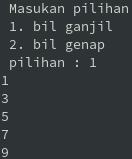
\includegraphics{1.png} 
    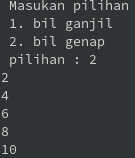
\includegraphics{2.png} 
\end{center}

\subsubsection{Praktik 2}
\begin{lstlisting}
import java.util.Scanner;

public class Praktik6_2 {
    public static void main(String args[]) {
        Scanner masuk = new Scanner(System.in);
        int pil, total, i;
        System.out.println(" Masukan pinjaman");
        System.out.println(" 1. Pembelian kredit");
        System.out.println(" 2. Pembelian tunai");
        System.out.print(" pilihan : ");
        pil = masuk.nextInt();
        System.out.print("total pembelian : ");
        total = masuk.nextInt();
        if (pil == 1) {
            if (total >= 1000000) {
                for (i = 1; i <= 10; i++) {
                    System.out.println("Angsuran ke =" + i + "sebesar " + (total / 10));
                }
            } else {
                for (i = 1; i <= 5; i++) {
                    System.out.println("Angsuran ke =" + i + "sebesar " + (total / 5));
                }
            }
        } else if (pil == 2) {
            System.out.println("Anda melakukan pembelian tunai");
        }
    }
}
\end{lstlisting}
Program praktik 2 di atas akan menghitung angsuran jika pembelian dilakukan secara kredit. Jika harga barang yang dibeli harganya lebih dari 1.000.000, maka angsuran akan dilakukan
10 kali, sedangkan jika yang dibeli harganya kurang dari 1.000.000 maka angsuran hanya akan dilakukan sebanyak 5 kali. Bila pembayaran dilakukan secara tunai, maka pembayaran harus dilakukan
dengan secara kontan.
\begin{center}
    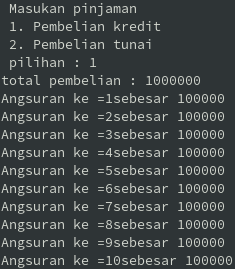
\includegraphics[scale=.8]{3.png}
    
\includegraphics[scale=.8]{4.png}
    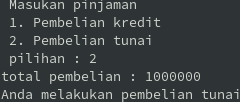
\includegraphics[scale=.8]{5.png}
\end{center}

\subsubsection{Praktik 3}
\begin{lstlisting}
import java.util.Scanner;

public class Praktik6_3 {
    public static void main(String args[]) {
        Scanner masuk = new Scanner(System.in);
        int pil, total, i;
        System.out.println("Masukan pinjaman");
        System.out.println("1. Pembelian kredit");
        System.out.println("2. Pembelian tunai");
        System.out.print("pilihan : ");
        pil = masuk.nextInt();
        System.out.print("total pembelian : ");
        total = masuk.nextInt();
        if (pil == 1) {
            if (total >= 1000000) {
                for (i = 1; i <= 10; i++) {
                    System.out.println("Angsuran ke =" + i + " sebesar " + (total / 10));
                }
            } else {
                for (i = 1; i <= 5; i++) {
                    System.out.println("Angsuran ke =" + i + " sebesar " + (total / 5));
                }
            }
        } else if (pil == 2) {
            if (total >= 1000000) {
                System.out.println("Anda melakukan pembelian tunai");
                double bayar = total - (0.05 * total);
                System.out.println("total bayar = " + bayar);
            } else {
                System.out.println("Anda melakukan pembelian tunai dan tidak mendapatkan diskon");
                System.out.println("Total yang harus dibayar " + total);
            }
        }
    }
}
\end{lstlisting}
Untuk praktik 3 adalah memodifikasi dari praktik 2. Pada praktik 3 ditambahkan seleksi pada else, sehingga jika pembeli membeli barang dengan harga 1.000.000, dan membayarnya dengan tunai,
maka pembeli akan mendapatkan diskon sebesar 5\%. Tetapi jika harga barang yang dibeli harganya di bawah 1.000.000, maka pembeli tidak mendapat diskon.
\begin{center}
    
\includegraphics[scale=.8]{6.png}
    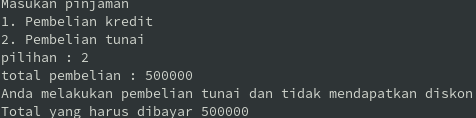
\includegraphics[scale=.8]{7.png}
\end{center}

\subsection{Latihan}
\subsubsection{Latihan 1}
\begin{lstlisting}
import java.util.Scanner;

public class Praktik6_1a {
    public static void main(String args[]) {
        Scanner masuk = new Scanner(System.in);
        int nilai, i;
        System.out.println(" Masukan pilihan");
        System.out.println(" 1. bil ganjil");
        System.out.println(" 2. bil genap");
        System.out.print(" pilihan : ");
        nilai = masuk.nextInt();
        if (nilai == 1) {
            i = 1;
            while (i <= 10) {
                System.out.println(i);
                i += 2;
            }
        } else {
            i = 2;
            while (i <= 10) {
                System.out.println(i);
                i += 2;
            }
        }
    }
}
\end{lstlisting}
Program java pada latihan 1, adalah program dari praktik 1 yang dimodifikasi perulangannya, yang semula memnggunakan perulangan for, dirubah menjadi perulangan while. Karena while tidak
memiliki fungsi increment, dan deklarasi variabel, maka variabel harus dideklarasikan sebelum perulangan, dan memberi pernyataan increment didalam while agar perulangan while dapat
berhenti.
\begin{center}
    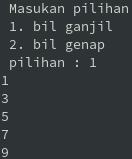
\includegraphics[scale=.8]{1.png}
    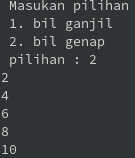
\includegraphics[scale=.8]{2.png}
\end{center}

\subsubsection{Latihan 2}
\begin{lstlisting}
import java.util.Scanner;

public class nilai {
    public static void main(String arg[]) {
        Scanner in = new Scanner(System.in);
        int nilai;
        System.out.print("Masukkan angka bulat (0 - 100) ");
        nilai = in.nextInt();
        if (nilai >= 60) {
            if (nilai >= 80)
                for (int i = 0; i < 5; i++) {
                    System.out.println("Nilaimu bagus sekali ");
                }
            else
                for (int i = 0; i < 5; i++) {
                    System.out.println("Nilaimu bagus ");
                }
        } else {
            if (nilai >= 30)
                for (int i = 0; i < 5; i++) {
                    System.out.println("Nilaimu kurang ");
                }
            else
                for (int i = 0; i < 5; i++) {
                    System.out.println("Nilaimu jelek ");
                }
        }
    }
}
\end{lstlisting}
Untuk latihan kedua, adalah menambahkan perulangan didalam seleksi, hasilnya program akan menampilkan kalimat sebanyak lima kali.
\begin{center}
    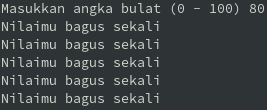
\includegraphics[scale=.8]{8.png}
    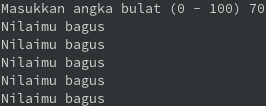
\includegraphics[scale=.8]{9.png}
    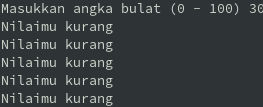
\includegraphics[scale=.8]{10.png}
    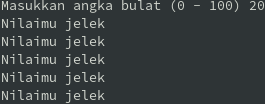
\includegraphics[scale=.8]{11.png}
\end{center}

\subsection{Tugas}
\begin{lstlisting}
import java.util.Scanner;

public class Tugas {
    public static void main(String[] args) {
        Scanner input = new Scanner(System.in);
        String matkul,jenjang;
        int sks, jumlah=0;
        System.out.print("Masukkan jenjang (D3/S1) = ");
        jenjang = input.nextLine();
        if (jenjang.equals("S1")){
            for(int i=0; i<5; i++){
                if(i>0){
                    input.nextLine();
                }
                System.out.print("Masukkan matakuliah = ");
                matkul = input.nextLine();
                System.out.print("Masukkan sks = ");
                sks = input.nextInt();
                jumlah = jumlah + sks;
            }
        }else{
            for(int i=0; i<3; i++){
                System.out.print("Masukkan matakuliah = ");
                if(i>0){
                    input.nextLine();
                }
                matkul = input.nextLine();
                System.out.print("Masukkan sks = ");
                sks = input.nextInt();
                jumlah = jumlah + sks;
            }
        }
        System.out.println("Total sks = "+jumlah);
    }
}
\end{lstlisting}
Program terssebut adalah program yang akan menghitung jumlah sks yang diambil oleh mahasiswa. Karena perulangan tersebut terdapat 2 input yang, maka ditambahkan seleksi untuk mencegah
input terlewati saat perulangan berjalan. untuk menjumlahkan sks yang dimasukkan, didalam perulangan ditambahkan jumlah = jumlah + sks.
\begin{center}
    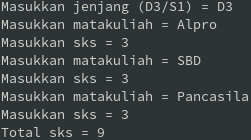
\includegraphics[scale=.8]{12.png} 
    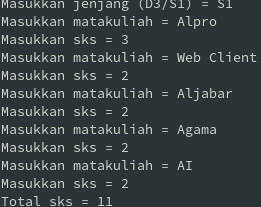
\includegraphics[scale=.8]{13.png} 
\end{center}

\newpage

\section{Kesimpulan}
Setelah praktik mahasiswa dapat menjelaskan konsep array 3 dimensi, merencanakan struktur data dalam bentuk array 3 dimensi, mengaplikasikan array 3 dimensi.

\end{document}
